% Section content template for individual Educative lessons
% This file contains the actual content for a specific section
% Generated from Educative API section content

% Section: Considerations of a Distributed Messaging Queue’s Design
% Section ID: 6191662786674688
% Section Slug: considerations-of-a-distributed-messaging-queues-design
% Generated: 2025-12-07T20:57:54.881342

Before embarking on our journey to design a distributed messaging queue, let's discuss some major factors that could significantly affect the design. These include the order of messages, the effect of the ordering on performance, and the management of concurrent access to the queue. We discuss each of these factors in detail below.

\subsection{Ordering of messages}\label{PMBDA01ByIIJuGPagf651}
\\
A messaging queue is used to receive messages from producers. These messages are consumed by the consumers at their own pace. Some operations are critical in that they require strict ordering of the execution of the tasks, driven by the messages in the queue. For example, while chatting over a messenger application with a friend, the messages should be delivered in order; otherwise, such communication can be confusing, to say the least. Similarly , emails received by a user from different users may not require strict ordering. Therefore, in some cases, the strict order of incoming messages in the queue is essential, while many use cases can tolerate some reordering.
\\
Let's discuss the following two categories of message ordering in a queue:

\begin{itemize}
\item
\protect\phantomsection\label{kRovk16FApPPQ2LJ-Rnn-}
\emph{Best-effort ordering}
\item
\protect\phantomsection\label{1iIDGIDr9r1q4PikQQ-Xm}
\emph{Strict ordering}
\end{itemize}

In a queue, the order of messages is implicitly associated with the incoming messages. Once the messages are put in a queue, the same order is followed in the consumption and processing of these messages.
\\
For concurrent producers putting messages in the same queue, the order is not well defined until producers provide order information---for example, timestamps or sequence numbers. Without any ordering information, the queue puts messages in the queue in whatever order they arrive at the service.
\\
For concurrent consumers fetching messages from the same queue, ordering can again become a complicated issue. While the queue can hand over messages one after the other in the same order as they were entered in the queue, two consumers almost concurrently processing two messages might need an application-specific ordering mechanism. The queue might help by tagging a message's ordering information, sequence number or timestamp, while handing out a message from the queue.

\subsubsection{Best-effort ordering}\label{3SZpNLdZDprIzMi6saDFU}
\\
With the \textbf{best-effort ordering} approach, the system puts the messages in a specified queue in the same order that they're received.
\\
For example, as shown in the following figure, the producer sends four messages, A, B, C, and D, in the same order as illustrated. Due to network congestion or some other issue, message B is received after message D. Hence , the order of messages is A, C, D, and B at the receiving end. Therefore, in this approach, the messages will be put in the queue in the same order they were received instead of the order in which they were produced on the client side.

\begin{figure}[htbp]
 \centering
 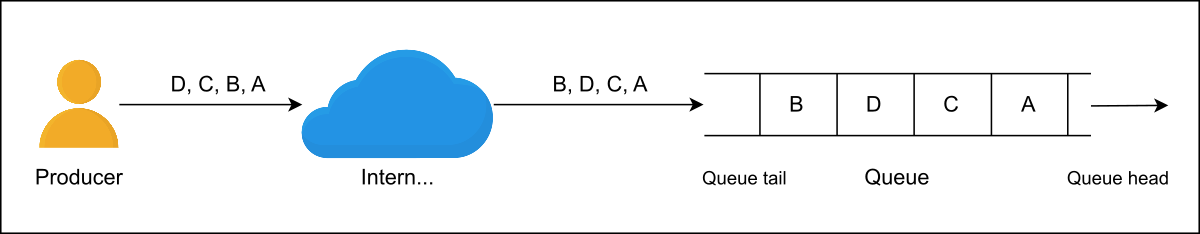
\includegraphics[width=0.5\textwidth]{Images/chapter_17/section_6191662786674688/4515921226104832.png}
 \caption{Best-effort ordering: Messages are placed in a queue in the same order that they’re received and not in the order they were sent}
\end{figure}

\subsubsection{Strict ordering}\label{_CUlnmQ_N-aeYA8oK-NWl}
\\
The strict ordering technique preserves the ordering of messages more rigorously. Through this approach, messages are placed in a queue in the order that they're produced.\\
\strut \\
Before putting messages in a queue in the correct sequence, it's crucial to have a mechanism to identify the order in which the messages were produced on the client side. Often , a unique identifier or time-stamp is used to mark a message when it's produced.\\

\begin{quote}
\textbf{Quiz:}
\textbf{Question 1:} Who'll be responsible for providing the sequence numbers?
\textbf{Answer:} The responsibility for providing sequence numbers lies with the client.

The system facilitates this by offering essential libraries or APIs that the client can integrate into their application. These tools allow the client to assign sequence numbers to messages as they are produced, ensuring each message can be tracked and ordered accurately. This approach helps maintain consistency and enables the system to process and deliver messages in the intended sequence.
\end{quote}

One of the following three approaches can be used for ordering incoming messages:

\begin{enumerate}
\item
\protect\phantomsection\label{7ZC98ODLFRoZaj7OL63yM}
\textbf{Monotonically increasing numbers:} One way to order incoming messages is to assign monotonically increasing numbers to messages on the server side. When the first message arrives, the system assigns it a number, such as 1. It then assigns the number 2 to the second message, and so on.\\
However, there are potential drawbacks to this approach. First , when a burst of requests is received, it acts as a bottleneck that affects the system's performance because the system has to assign an ID in a specified sequence to a message while the other messages wait for their turn.\\
Second, it still doesn't tackle the problem that arises when a message is received before the one that's produced earlier at the client side. Because of this, it doesn't guarantee that it will generate the correct order for the messages produced at the client side.
\item
\protect\phantomsection\label{gAeco2jyusyxo8OYN6iNX}
\textbf{Causality-based sorting at the server side:} Keeping in view the drawbacks of using monotonically increasing numbers, another approach that can be used for time-stamping and ordering of incoming messages is causality-based sorting. In this approach, messages are sorted based on the time stamp that was produced at the client side and are put in a queue accordingly. The major drawback of this approach is that for multiple client sessions, the service can't determine the order in terms of wall-clock time.
\item
\protect\phantomsection\label{_ZXJ_-nTM59BSBPZlC3xW}
\textbf{Using time stamps based on synchronized clocks:} To tackle the potential issues that arise with both of the approaches described above, we can use another appropriate method to assign time stamps to messages that's based on synchronized clocks. In this approach, the time stamp (ID) provided to each message through a synchronized clock is unique and in the correct sequence of production of messages. We can tag a unique process identifier with the time stamp to make the overall message identifier unique and tackle the situation when two concurrent sessions ask for a time stamp at the exact same time. Moreover, with this approach, the server can easily identify delayed messages based on the time stamp and wait for the delayed messages.\\
As we discussed in the section on the \href{https://www.educative.io/courses/grokking-the-system-design-interview/system-design-sequencer}{sequencer} building block, we can get sequence numbers that fulfill double duty as sequence numbers and globally synchronized wall clock time stamps. Using this approach, our service can globally order messages across client sessions as well.
\end{enumerate}
\\
To conclude, the most appropriate mechanism to provide a unique ID or time stamp to incoming messages, from among the three approaches described above, involves the use of synchronized clocks.
\\
\paragraph{Sorting}\label{vSNEXYECZ2Tw5t4JFFB2K}
\\
Once messages are received at the server side, we need to sort them based on their time stamps. Therefore, we use an appropriate online sorting(Online sorting means that we need to keep some data sorted as new data keeps coming in.) algorithm for this purpose.

\begin{quote}
\textbf{Quiz:}
\textbf{Question 1:} Suppose that a message sent earlier arrives late due to a network delay.

What would be the proper approach to handle such a situation?
\textbf{Answer:} The simple solution in such cases is to reorder the queue. Two scenarios can arise from this. First, reordering puts the messages in the correct order. Second, we've already handed out newer messages to the consumers.

If an old message comes when we've already handed out a newer message, we put it in a special queue, and the client handles that situation. The client may later decide whether to consume the message if the message does not affect the intended operation or discard it if it\textquotesingle s not needed.
\end{quote}

\subsection{Effect on performance}\label{y2V-TK0AkiwMnQUAS6RM8}
\\
Primarily, a queue is designed for first-in, \textbf{first-out (FIFO) operations};. First-in, first-out operations suggest that the first message that enters a queue is always handed out first. However, it isn't easy to maintain this strict order in distributed systems. Since message A was produced before message B, it's still uncertain that message A will be consumed before message B. Using monotonically increasing message identifiers or causality-bearing identifiers provide high throughput while putting messages in a queue. Though the need for the online sorting to provide a strict order takes some time before messages are ready for extraction. To minimize latency caused by the online sorting, we use a \textbf{time-window}(We have to sort messages received within a specific time frame and then put them in the relevant queue (the oldest will be the first to be put in the queue).) approach.
\\
Similarly, for strict ordering at the receiving end, we need to serialize all the requests to give out messages one by one. If that's not required, we have better throughput and lower latency at the receiving end.
\\
Due to the reasons mentioned above, many distributed messaging queue solutions either don't guarantee a strict order or have limitations around throughput. As we saw previously, the queues have to perform many additional validations and coordination operations to maintain the order.

\subsubsection{Managing concurrency}\label{tVHkbhrOWconzbR0XT_ep}
\\
Concurrent queue access needs proper management. Concurrency can take place at the following stages:

\begin{itemize}
\item
\protect\phantomsection\label{Jk1GCN_tsWfNLIQaAUsW3}
When multiple messages arrive at the same time.
\item
\protect\phantomsection\label{sMCjiNFRocd5IOA1-scE3}
When multiple consumers request concurrently for a message.
\end{itemize}
\\
The first solution is to use the locking mechanism. When a process or thread requests a message, it should acquire a lock for placing or consuming messages from the queue. However, as was discussed earlier, this approach has several drawbacks. It's neither scalable nor performant.
\\
Another solution is to serialize the requests using the system's buffer at both ends of the queue so that the incoming messages are placed in an order, and consumer processes also receive messages in their arrival sequence. By serializing requests, we mean that the requests (either for putting data or extracting data), which come to the server would be queued by the OS, and a single application thread will put them in the queue (we can assume that both kinds of requests, put and extract come to the same port) without any locking. It will be a possible lock-free solution, providing high throughput. This is a more viable solution because it can help us avoid the occurrence of race conditions.
\\
Applications might use multiple queues with dedicated producers and consumers to keep the ordering cost per queue under check, although this comes at the cost of more complicated application logic.

\begin{figure}[htbp]
 \centering
 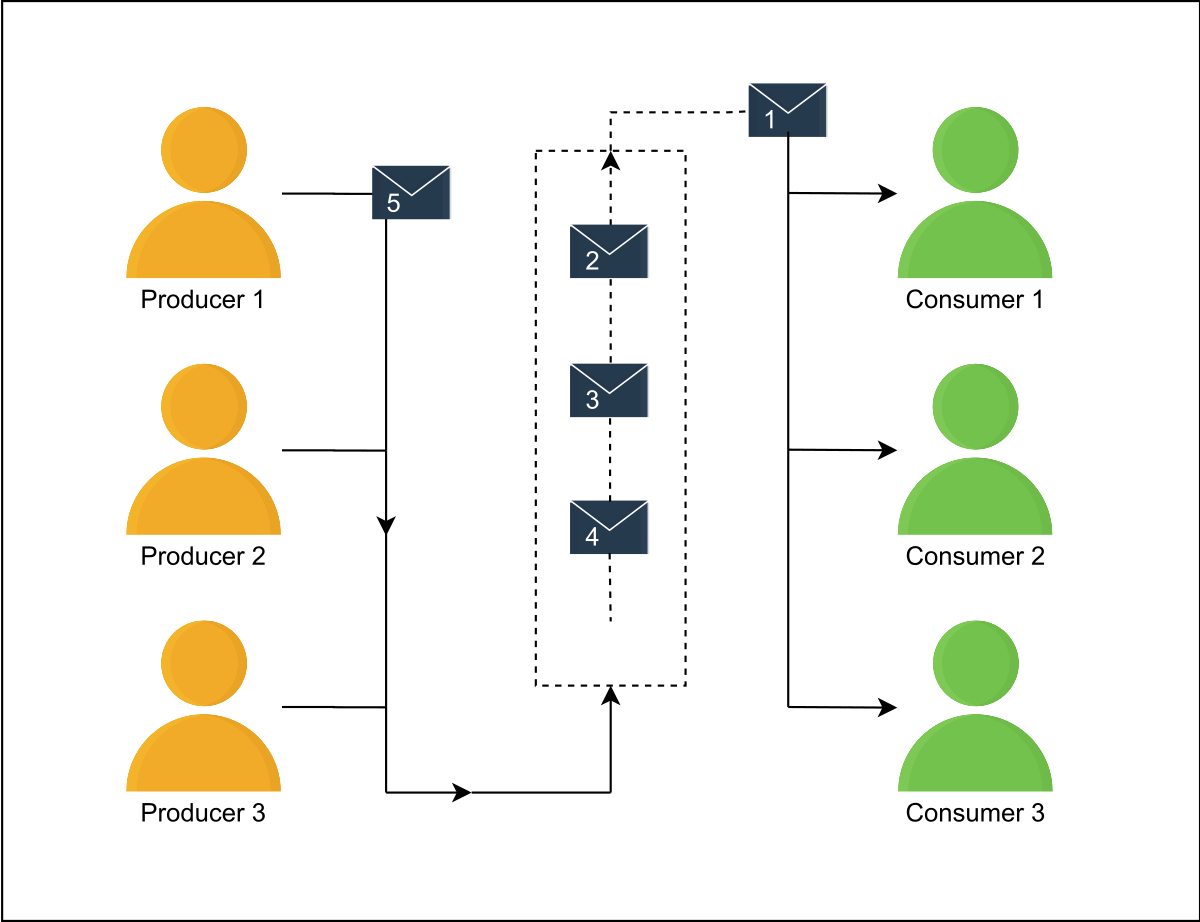
\includegraphics[width=0.5\textwidth]{Images/chapter_17/section_6191662786674688/5678750335500288.png}
 \caption{Avoiding race conditions: Producers and consumers are serialized at both ends of the queue}
\end{figure}

In this lesson, we discussed some key considerations and challenges in the design process of a messaging queue and answered the following questions:

\begin{itemize}
\item
\protect\phantomsection\label{2VfPYwn0bTDjKiXvlZ9JV}
Why is the order of messages important, and how do we enforce that order?
\item
\protect\phantomsection\label{ToVMGrgnb8rVNoGQZCPK9}
How does ordering affect performance? How do we handle concurrency while accessing a queue?
\end{itemize}
\\
Now, we are ready to start designing a distributed messaging queue.

% End of section content